% !TeX root = enterprise-architecture-digital-blueprint.tex
% !TeX encoding = UTF-8
\chapter{Pemodelan Arsitektur dengan ArchiMate dan Archi}

\section*{Tujuan Pembelajaran}
\begin{itemize}
  \item Menjelaskan kerangka inti ArchiMate: lapisan, aspek, elemen, dan relasi.
  \item Membangun model berlapis di Archi yang menghubungkan layanan bisnis, proses, aplikasi, dan teknologi.
  \item Memilih \textit{viewpoint} yang sesuai dengan \textit{concern} pemangku kepentingan tertentu.
\end{itemize}

\section{Pendahuluan}

Hampir setiap rapat proyek TI memakai gambar kotak dan panah. Masalahnya,
gambar yang sama dibaca berbeda oleh tiap orang. Bagi kepala keuangan, panah
dari ``SIMRS'' ke ``ERP'' berarti tagihan pasien mengalir ke pembukuan. Bagi
tim integrasi, panah yang sama berarti ERP memanggil SIMRS setiap malam.
Bagi vendor, panah itu mungkin berarti tidak ada apa-apa, karena gambarnya
dibuat orang lain. Tiga pembaca, tiga arti, dan tidak ada yang salah menurut
gambarnya sendiri.

Masalah kedua muncul ketika gambar yang sama digambar ulang di banyak
dokumen. Proposal vendor, laporan audit, dan bahan presentasi direksi
masing-masing punya versi sendiri. Nama sistem berbeda, kotak yang
digambar berbeda, dan ketika satu sistem diganti, hanya sebagian gambar yang
ikut diperbarui. Setelah dua atau tiga tahun, organisasi punya puluhan gambar
arsitektur yang saling bertentangan, dan tidak ada yang tahu gambar mana yang
benar.

Bab ini menjawab kedua masalah itu dengan bahasa pemodelan yang punya arti
baku, yaitu ArchiMate 3.2 \cite{archimate32}, dan alat pemodelan gratis Archi
5.10.0 yang mendukungnya \cite{archi}. Pembahasan dimulai dari perbedaan
model dan gambar, lalu masuk ke kerangka inti ArchiMate, relasi, dan
\textit{viewpoint} yang mengikat konsep \textit{stakeholder}, \textit{concern},
dan \textit{view} dari ISO/IEC/IEEE 42010:2022 \cite{iso42010} seperti dibahas
di Bab 2. Bab ini ditutup dengan perubahan pada ArchiMate 4 yang terbit April
2026 \cite{archimate4}. Buku Lankhorst \cite{lankhorst2017} dipakai sebagai
bacaan pendamping untuk pemodelan, komunikasi, dan analisis arsitektur.

\section{Model, Diagram, dan Repositori}

Model arsitektur adalah kumpulan elemen dan relasi yang masing-masing punya
arti baku. Elemen ``SIMRS RS Bekasi'' di dalam model bukan sekadar kotak
bertuliskan nama, melainkan sebuah komponen aplikasi yang punya pemilik,
status, dan hubungan dengan proses yang dilayaninya. Diagram, yang dalam
ArchiMate disebut \textit{view}, hanyalah gambar yang menampilkan sebagian
isi model untuk pembaca tertentu. Repositori adalah tempat model dan seluruh
\textit{view}-nya disimpan, sehingga menjadi satu sumber rujukan bagi
seluruh tim. Satu elemen cukup dibuat sekali di repositori, lalu dipakai di
banyak \textit{view}. Notasi yang artinya baku juga membuat gambar lebih
mudah dibaca dengan cara yang sama oleh orang yang berbeda \cite{c04-moody2009}.

Analoginya seperti buku kontak di ponsel. Nomor seorang teman disimpan sekali
di buku kontak, lalu muncul di banyak grup percakapan. Ketika teman itu
berganti nomor, cukup satu kontak yang diubah, dan seluruh grup langsung
memakai nomor baru. Bayangkan bila tiap grup menyimpan daftar nomornya
sendiri di catatan terpisah. Setelah beberapa kali ganti nomor, tidak ada yang
tahu nomor mana yang masih berlaku.

Gambar \ref{fig:ch04-model-view} memperlihatkan perbedaan kedua cara kerja
itu untuk satu sistem yang sama.

\begin{figure}[!htb]
  \centering
  \begin{tikzpicture}[
  font=\scriptsize,
  kotak/.style={draw, rounded corners, minimum height=0.85cm, minimum width=2.9cm,
                align=center, font=\scriptsize\bfseries},
  panah/.style={-{Stealth[length=2mm]}, thick}
]
  % Panel kiri: setiap dokumen menggambar ulang sistem yang sama.
  \node[font=\footnotesize\bfseries] at (2.4,2.45) {Hanya menggambar};
  \node[kotak, fill=red!22] (g1) at (2.4,1.4)
    {Proposal vendor\\{\tiny\mdseries ``SIMRS Bekasi v4''}};
  \node[kotak, fill=red!22] (g2) at (2.4,0.2)
    {Laporan audit\\{\tiny\mdseries ``Sistem RS Bekasi''}};
  \node[kotak, fill=red!22] (g3) at (2.4,-1.0)
    {Presentasi direksi\\{\tiny\mdseries ``HIS Bekasi''}};
  \node[font=\tiny, gray, align=center] at (2.4,-1.95)
    {tiga gambar, tiga nama,\\tidak saling tahu bila sistemnya berubah};

  \draw[gray, dashed] (4.75,2.7) -- (4.75,-2.3);

  % Panel kanan: satu elemen di repositori dipakai oleh banyak view.
  \node[font=\footnotesize\bfseries] at (8.3,2.45) {Memodelkan};
  \node[kotak, fill=praditagreen!15, minimum height=2.9cm, minimum width=2.6cm] (repo)
    at (6.55,0.2)
    {Repositori model\\[3pt]{\tiny\mdseries satu elemen:}\\SIMRS RS Bekasi\\
     {\tiny\mdseries komponen aplikasi}};
  \node[kotak, fill=blue!8] (v1) at (10.3,1.4)
    {Layered view\\{\tiny\mdseries untuk tim TI}};
  \node[kotak, fill=blue!8] (v2) at (10.3,0.2)
    {Application cooperation\\{\tiny\mdseries untuk tim integrasi}};
  \node[kotak, fill=green!10] (v3) at (10.3,-1.0)
    {View layanan pasien\\{\tiny\mdseries untuk direksi}};

  \draw[panah] ($(repo.east)+(0,0.6)$) -- (v1.west);
  \draw[panah] (repo.east) -- (v2.west);
  \draw[panah] ($(repo.east)+(0,-0.6)$) -- (v3.west);
  \node[font=\tiny, gray, align=center] at (8.3,-1.95)
    {ubah sekali di repositori,\\semua view ikut berubah};
\end{tikzpicture}

  \caption{Hanya menggambar menghasilkan banyak versi yang tidak saling tahu,
           sedangkan memodelkan menyimpan satu elemen yang dipakai di banyak
           \textit{view}}
  \label{fig:ch04-model-view}
\end{figure}

Dua contoh dari Medikara Health:

\begin{enumerate}
  \item Misalkan tim arsitektur Medikara mengumpulkan seluruh gambar
        arsitektur yang dibuat antara 2021 dan 2025. Hasilnya 46 gambar di 19
        dokumen. SIMRS RS Bekasi muncul di 14 gambar dengan 4 nama berbeda:
        ``SIMRS Bekasi v4'', ``Sistem RS Bekasi'', ``HIS Bekasi'', dan
        ``SIMRS RS Bekasi''. Pembaca baru tidak dapat memastikan apakah
        keempatnya sistem yang sama.
  \item Misalkan SIMRS RS Bekasi diganti pada 2027. Tanpa model, 14 gambar
        harus dicari dan digambar ulang satu per satu. Dengan model, tim
        mengubah satu elemen, lalu menelusuri relasinya untuk menjawab
        pertanyaan dampak: proses mana yang dilayani sistem itu, data apa yang
        disimpannya, dan server mana yang menjalankannya.
\end{enumerate}

Tabel \ref{tab:ch04-model-gambar} merangkum perbedaan kedua cara kerja itu.

\begin{table}[!htb]
  \centering
  \caption{Hanya menggambar dibandingkan dengan memodelkan di repositori}
  \label{tab:ch04-model-gambar}
  \begin{tabularx}{\textwidth}{lXX}
    \hline
    \textbf{Aspek} & \textbf{Hanya menggambar} & \textbf{Memodelkan di repositori} \\
    \hline
    Tempat arti & Di kepala pembuat gambar & Di elemen dan relasi yang artinya baku \\
    \hline
    Perubahan & Setiap gambar diubah satu per satu & Satu elemen diubah, semua \textit{view} ikut \\
    \hline
    Konsistensi nama & Bergantung pada ketelitian tiap penulis & Satu nama per elemen \\
    \hline
    Analisis dampak & Membaca ulang seluruh dokumen & Menelusuri relasi elemen \\
    \hline
    Biaya awal & Rendah, cukup alat gambar & Lebih tinggi: belajar bahasa, alat, dan konvensi \\
    \hline
  \end{tabularx}
\end{table}

Keputusan untuk hanya menggambar punya dua konsekuensi. Pertama, biaya
pemeliharaan tumbuh mengikuti jumlah gambar, bukan jumlah sistem. Sepuluh
sistem yang masing-masing muncul di lima gambar berarti 50 tempat yang harus
diperbarui. Kedua, pertanyaan analisis seperti ``apa yang terdampak bila
sistem ini mati'' tidak dapat dijawab dari gambar, karena gambar tidak
menyimpan hubungan, hanya garis.

Dua hal pada repositori sering tertukar. Pembagiannya begini. Menghapus
elemen dari sebuah \textit{view} hanya menghapus gambarnya, sedangkan
elemennya tetap ada di model dan di \textit{view} lain. Menghapus elemen dari
model menghapusnya dari seluruh \textit{view} sekaligus. Archi membedakan
keduanya dengan jelas: penghapusan di kanvas \textit{view} hanya menyentuh
\textit{view} itu, sedangkan penghapusan di pohon model menyentuh seluruh
model.

\section{Kerangka Inti ArchiMate}

ArchiMate adalah bahasa pemodelan arsitektur \textit{enterprise} yang
diterbitkan The Open Group \cite{archimate32}. Inti bahasanya berupa kisi tiga
kali tiga. Arah mendatar berisi tiga lapisan: bisnis (layanan kepada pasien
dan mitra, proses, serta pelakunya), aplikasi (aplikasi dan data), dan
teknologi (server, jaringan, perangkat lunak sistem, serta perangkat
fisik). Arah menurun berisi tiga aspek: struktur aktif (siapa atau apa yang
mengerjakan), perilaku (apa yang dikerjakan), dan struktur pasif (apa yang
dikenai pekerjaan). Lapisan yang lebih bawah melayani lapisan di atasnya
lewat layanan. Di luar kisi inti, ArchiMate menambahkan elemen strategi,
elemen motivasi, serta elemen implementasi dan migrasi. Gambar
\ref{fig:ch04-kerangka-inti} memperlihatkan susunannya beserta contoh dari
layanan janji temu Medikara.

\begin{figure}[!htb]
  \centering
  \begin{tikzpicture}[
  font=\scriptsize,
  sel/.style={draw, rounded corners, minimum height=1.05cm, minimum width=2.7cm,
              text width=2.5cm, align=center, font=\scriptsize\bfseries},
  label/.style={draw, rounded corners, fill=praditagreen!15, align=center,
                font=\scriptsize\bfseries},
  panah/.style={-{Stealth[length=2mm]}, thick}
]
  % Judul kolom: tiga aspek inti, ditambah aspek motivasi di kanan.
  \node[label, minimum width=2.7cm, minimum height=0.6cm] at (2.95,3.55) {Struktur pasif};
  \node[label, minimum width=2.7cm, minimum height=0.6cm] at (5.75,3.55) {Perilaku};
  \node[label, minimum width=2.7cm, minimum height=0.6cm] at (8.55,3.55) {Struktur aktif};

  % Lapisan strategi di atas inti.
  \node[sel, fill=blue!8, minimum width=8.3cm, text width=8.1cm, minimum height=0.75cm]
    at (5.75,2.6)
    {Strategi: kapabilitas, \textit{value stream}, sumber daya, \textit{course of action}};

  % Judul baris: tiga lapisan inti.
  \node[label, minimum width=1.5cm, minimum height=1.05cm] at (0.75,1.5) {Bisnis};
  \node[label, minimum width=1.5cm, minimum height=1.05cm] at (0.75,0.3) {Aplikasi};
  \node[label, minimum width=1.5cm, minimum height=1.05cm] at (0.75,-0.9) {Teknologi};

  % Isi inti 3 x 3, dengan contoh dari layanan janji temu Medikara.
  \node[sel, fill=orange!12] at (2.95,1.5)
    {Objek bisnis\\{\tiny\mdseries Janji Temu}};
  \node[sel, fill=orange!12] at (5.75,1.5)
    {Proses, fungsi, layanan bisnis\\{\tiny\mdseries Membuat Janji Temu}};
  \node[sel, fill=orange!12] at (8.55,1.5)
    {Aktor, peran\\{\tiny\mdseries Pasien, Petugas Pendaftaran}};

  \node[sel, fill=orange!12] at (2.95,0.3)
    {Objek data\\{\tiny\mdseries Data Jadwal Dokter}};
  \node[sel, fill=orange!12] at (5.75,0.3)
    {Fungsi, layanan aplikasi\\{\tiny\mdseries Layanan Pemesanan Jadwal}};
  \node[sel, fill=orange!12] at (8.55,0.3)
    {Komponen, antarmuka\\{\tiny\mdseries Medikara+, SIMRS}};

  \node[sel, fill=orange!12] at (2.95,-0.9)
    {Artefak\\{\tiny\mdseries berkas basis data}};
  \node[sel, fill=orange!12] at (5.75,-0.9)
    {Layanan teknologi\\{\tiny\mdseries Layanan Basis Data}};
  \node[sel, fill=orange!12] at (8.55,-0.9)
    {\textit{Node}, perangkat\\{\tiny\mdseries Server Basis Data SIMRS}};

  % Aspek motivasi di sisi kanan, merentang seluruh lapisan.
  \node[sel, fill=blue!8, minimum width=1.8cm, text width=1.6cm, minimum height=4.35cm]
    at (11.0,0.3)
    {Motivasi\\[3pt]{\tiny\mdseries \textit{stakeholder}, \textit{driver}, \textit{goal},
     \textit{outcome}, prinsip, \textit{requirement}}};

  % Lapisan implementasi dan migrasi di bawah inti.
  \node[sel, fill=blue!8, minimum width=8.3cm, text width=8.1cm, minimum height=0.75cm]
    at (5.75,-2.0)
    {Implementasi dan migrasi: \textit{work package}, \textit{deliverable}, \textit{plateau}, \textit{gap}};

  \node[font=\tiny, gray, anchor=north] at (5.75,-2.45)
    {kotak oranye: kerangka inti tiga lapisan kali tiga aspek};
\end{tikzpicture}

  \caption{Kerangka inti ArchiMate 3.2: tiga lapisan kali tiga aspek, diapit
           elemen strategi, motivasi, serta implementasi dan migrasi}
  \label{fig:ch04-kerangka-inti}
\end{figure}

Analoginya seperti pelajaran SPOK di sekolah dasar. Kalimat ``Petugas
pendaftaran mencatat janji temu'' terdiri atas subjek (petugas pendaftaran),
predikat (mencatat), dan objek (janji temu). Struktur aktif adalah subjek,
perilaku adalah predikat, dan struktur pasif adalah objek. Lapisan aplikasi
memakai pola kalimat yang sama: ``SIMRS mengelola data jadwal dokter''.
Kalimat tanpa predikat tidak bermakna, dan model tanpa elemen perilaku juga
tidak menjelaskan apa yang terjadi.

Setiap lapisan juga punya sisi dalam dan sisi luar. Sisi luar adalah apa yang
dilihat pemakai: layanan (\textit{service}) dan antarmuka
(\textit{interface}). Sisi dalam adalah cara layanan itu diwujudkan: proses,
fungsi, dan komponen. Pasien tidak peduli proses apa yang terjadi di balik
layanan janji temu. Pasien hanya peduli bahwa slot dokter didapat tanpa antre.
Karena itu layanan selalu menjadi titik sambung yang paling penting, baik
antara organisasi dan pelanggannya maupun antara satu lapisan dan lapisan di
atasnya.

ArchiMate 3.2 memuat puluhan jenis elemen. Cetak biru di mata kuliah ini
cukup memakai belasan, seperti pada Tabel \ref{tab:ch04-elemen}. Nama Inggris
ditulis karena Archi memakai nama itu di palet dan pohon modelnya.

\begin{table}[!htb]
  \centering
  \caption{Elemen ArchiMate 3.2 yang paling sering dipakai di cetak biru
           \textit{capstone}}
  \label{tab:ch04-elemen}
  \small
  \begin{tabularx}{\textwidth}{>{\raggedright\arraybackslash}p{3.3cm}lX}
    \hline
    \textbf{Elemen} & \textbf{Lapisan dan aspek} & \textbf{Contoh Medikara} \\
    \hline
    Aktor bisnis (\textit{business actor}) & Bisnis, aktif & Pasien, BPJS Kesehatan \\
    \hline
    Peran bisnis (\textit{business role}) & Bisnis, aktif & Petugas Pendaftaran \\
    \hline
    Proses bisnis (\textit{business process}) & Bisnis, perilaku & Membuat Janji Temu \\
    \hline
    Layanan bisnis (\textit{business service}) & Bisnis, perilaku & Layanan Janji Temu Rawat Jalan \\
    \hline
    Objek bisnis (\textit{business object}) & Bisnis, pasif & Janji Temu \\
    \hline
    Komponen aplikasi (\textit{application component}) & Aplikasi, aktif & Medikara+, SIMRS RS Jakarta \\
    \hline
    Fungsi aplikasi (\textit{application function}) & Aplikasi, perilaku & Pengelolaan Jadwal Dokter \\
    \hline
    Layanan aplikasi (\textit{application service}) & Aplikasi, perilaku & Layanan Pemesanan Jadwal \\
    \hline
    Objek data (\textit{data object}) & Aplikasi, pasif & Data Jadwal Dokter \\
    \hline
    \textit{Node} & Teknologi, aktif & Server Basis Data SIMRS \\
    \hline
    Perangkat lunak sistem (\textit{system software}) & Teknologi, aktif & Sistem Manajemen Basis Data \\
    \hline
    Layanan teknologi (\textit{technology service}) & Teknologi, perilaku & Layanan Basis Data \\
    \hline
    Kapabilitas (\textit{capability}) & Strategi & Penjadwalan Layanan Pasien \\
    \hline
    \textit{Driver}, \textit{goal}, \textit{outcome}, \textit{requirement} & Motivasi & Antrean Layanan yang Panjang \\
    \hline
    \textit{Work package}, \textit{plateau} & Implementasi dan migrasi & Konsolidasi SIMRS \\
    \hline
  \end{tabularx}
\end{table}

Pertanyaan kemudian muncul: bagaimana ketiga lapisan disambung? Jawabannya
selalu lewat layanan. Layanan aplikasi melayani proses bisnis, dan layanan
teknologi melayani komponen aplikasi. Dua contoh dari Medikara:

\begin{enumerate}
  \item Proses Membuat Janji Temu dilayani Layanan Pemesanan Jadwal milik
        Medikara+. Bila layanan aplikasi ini mati, janji temu tetap dapat
        dibuat lewat telepon dan loket, tetapi seluruh beban pindah ke
        petugas pendaftaran di lima rumah sakit dan 18 klinik pratama.
  \item SIMRS RS Jakarta dilayani Layanan Basis Data yang berjalan di satu
        server \textit{on-premise}. Satu server itu
        menopang seluruh jadwal dokter RS Jakarta, sehingga model langsung
        menunjukkan titik tunggal kegagalan yang perlu dibahas di Bab 7.
\end{enumerate}

Tiga kelompok elemen di luar kisi inti dipakai di bab-bab berikutnya. Elemen
strategi, terutama kapabilitas dan \textit{value stream}, menjadi bahan Bab 5.
Elemen motivasi sudah dikenal dari rantai motivasi di Bab 3, dan bab ini
memindahkannya ke dalam model. Elemen implementasi dan migrasi, seperti
\textit{work package} dan \textit{plateau}, dipakai di Bab 11 dan Bab 12.

\begin{kasus}[title={Kasus Medikara Health: Layanan Janji Temu dari Pasien sampai Server}]
  Layanan janji temu rawat jalan dipilih karena menyentuh tiga pemicu
  strategi sekaligus: antrean yang panjang, data pasien yang tersebar, dan
  integrasi \textit{point-to-point} antara Medikara+ dan lima SIMRS.
  Gambar \ref{fig:ch04-layered-janji-temu} memetakan layanan itu ke tiap
  lapisan.

  \begin{itemize}
    \item \textbf{Bisnis.} Pasien dilayani Layanan Janji Temu Rawat Jalan.
          Layanan itu diwujudkan proses Membuat Janji Temu, yang menulis
          objek bisnis Janji Temu.
    \item \textbf{Aplikasi.} Proses itu dilayani Layanan Pemesanan Jadwal
          yang diwujudkan Medikara+. Medikara+ membaca jadwal dari SIMRS RS
          Jakarta, yang menyimpan Data Jadwal Dokter.
    \item \textbf{Teknologi.} SIMRS RS Jakarta dilayani Layanan Basis Data
          yang diwujudkan Server Basis Data SIMRS.
  \end{itemize}

  Model lengkapnya tersedia di
  \berkas{sources/chapter04/medikara-janji-temu.archimate}. Isinya 26
  elemen, 30 relasi, dan tiga \textit{view}. Gambar di bawah adalah
  ringkasan \textit{layered view} model itu. Pemetaan ini baru mencakup satu
  dari lima rumah sakit. Empat SIMRS lain akan menambah empat komponen
  aplikasi, empat server, dan empat integrasi, dan itulah yang
  dipotret di Bab 7.
\end{kasus}

\begin{figure}[!htb]
  \centering
  \begin{tikzpicture}[
  font=\scriptsize,
  elemen/.style={draw, rounded corners=1pt, minimum height=0.8cm, minimum width=3.0cm,
                 align=center, font=\scriptsize\bfseries, fill=blue!8},
  panah/.style={-{Stealth[length=2mm]}, thick},
  layani/.style={-{Straight Barb[length=2mm, width=2.4mm]}, thick},
  realisasi/.style={-{Triangle[open, length=2.2mm, width=2.4mm]}, thick, dashed},
  akses/.style={-{Straight Barb[length=1.4mm, width=1.8mm]}, thick, dotted}
]
  % Pita lapisan.
  \draw[gray, dashed] (-0.9,2.05) -- (10.6,2.05);
  \draw[gray, dashed] (-0.9,-0.65) -- (10.6,-0.65);
  \node[rotate=90, font=\scriptsize\bfseries, text=praditagreen] at (-0.6,3.3) {Bisnis};
  \node[rotate=90, font=\scriptsize\bfseries, text=praditagreen] at (-0.6,0.7) {Aplikasi};
  \node[rotate=90, font=\scriptsize\bfseries, text=praditagreen] at (-0.6,-1.9) {Teknologi};

  % Lapisan bisnis.
  \node[elemen, fill=green!10, minimum width=2.2cm] (pasien) at (1.3,3.9)
    {Pasien\\{\tiny\mdseries aktor bisnis}};
  \node[elemen] (layjanji) at (5.0,3.9)
    {Layanan Janji Temu\\Rawat Jalan {\tiny\mdseries (layanan bisnis)}};
  \node[elemen] (proses) at (5.0,2.65)
    {Membuat Janji Temu\\{\tiny\mdseries proses bisnis}};
  \node[elemen] (objek) at (9.0,2.65)
    {Janji Temu\\{\tiny\mdseries objek bisnis}};

  % Lapisan aplikasi.
  \node[elemen, fill=orange!12] (laypesan) at (5.0,1.3)
    {Layanan Pemesanan Jadwal\\{\tiny\mdseries layanan aplikasi}};
  \node[elemen] (medikara) at (5.0,0.05)
    {Medikara+\\{\tiny\mdseries komponen aplikasi}};
  \node[elemen] (simrs) at (9.0,0.05)
    {SIMRS RS Jakarta\\{\tiny\mdseries komponen aplikasi}};
  \node[elemen] (data) at (9.0,1.3)
    {Data Jadwal Dokter\\{\tiny\mdseries objek data}};

  % Lapisan teknologi.
  \node[elemen, fill=orange!12] (laydb) at (9.0,-1.3)
    {Layanan Basis Data\\{\tiny\mdseries layanan teknologi}};
  \node[elemen] (server) at (9.0,-2.55)
    {Server Basis Data SIMRS\\{\tiny\mdseries \textit{node}}};

  % Relasi.
  \draw[layani] (layjanji) -- (pasien);
  \draw[realisasi] (proses) -- (layjanji);
  \draw[akses] (proses) -- (objek);
  \draw[layani] (laypesan) -- (proses);
  \draw[realisasi] (medikara) -- (laypesan);
  \draw[layani] (simrs) -- (medikara);
  \draw[akses] (simrs) -- (data);
  \draw[layani] (laydb) -- (simrs);
  \draw[realisasi] (server) -- (laydb);

  % Keterangan notasi.
  \draw[layani] (0.0,-3.55) -- (0.9,-3.55);
  \node[anchor=west, font=\tiny] at (1.0,-3.55) {melayani};
  \draw[realisasi] (2.5,-3.55) -- (3.4,-3.55);
  \node[anchor=west, font=\tiny] at (3.5,-3.55) {merealisasikan};
  \draw[akses] (5.4,-3.55) -- (6.3,-3.55);
  \node[anchor=west, font=\tiny] at (6.4,-3.55) {mengakses (menulis)};
  \node[anchor=west, font=\tiny, gray] at (0.0,-1.3)
    {kotak oranye: titik sambung antarlapisan};
\end{tikzpicture}

  \caption{\textit{Layered view} layanan janji temu rawat jalan Medikara, dari
           pasien sampai server basis data SIMRS}
  \label{fig:ch04-layered-janji-temu}
\end{figure}

\section{Relasi dan Aturan Pemakaiannya}

Relasi adalah penghubung antarelemen yang artinya ditetapkan oleh
spesifikasi. ArchiMate 3.2 membagi relasi menjadi empat kelompok
\cite{archimate32}. Relasi struktural menyatakan susunan: komposisi,
agregasi, penugasan, dan realisasi. Relasi dependensi menyatakan
ketergantungan: melayani, akses, pengaruh, dan asosiasi. Relasi dinamis
menyatakan urutan dan perpindahan: pemicu dan aliran. Kelompok terakhir
berisi spesialisasi. Setiap relasi punya arah, dan relasi dibaca sebagai
kalimat dari sumber ke tujuan: ``Layanan Pemesanan Jadwal melayani Membuat
Janji Temu''. Gambar \ref{fig:ch04-notasi-relasi} memperlihatkan notasinya.

\begin{figure}[!htb]
  \centering
  \begin{tikzpicture}[
  font=\scriptsize,
  judul/.style={draw, rounded corners, fill=praditagreen!15, minimum height=0.55cm,
                minimum width=5.5cm, font=\scriptsize\bfseries},
  ket/.style={anchor=west, align=left, font=\scriptsize\bfseries},
  panah/.style={-{Stealth[length=2mm]}, thick},
  komposisi/.style={{Diamond[length=3mm, width=2mm]}-, thick},
  agregasi/.style={{Diamond[open, length=3mm, width=2mm]}-, thick},
  penugasan/.style={{Circle[length=1.6mm]}-{Stealth[length=2mm]}, thick},
  realisasi/.style={-{Triangle[open, length=2.2mm, width=2.4mm]}, thick, dashed},
  layani/.style={-{Straight Barb[length=2mm, width=2.4mm]}, thick},
  akses/.style={-{Straight Barb[length=1.4mm, width=1.8mm]}, thick, dotted},
  pengaruh/.style={-{Straight Barb[length=2mm, width=2.4mm]}, thick, dashed},
  asosiasi/.style={thick},
  pemicu/.style={-{Triangle[length=2.2mm, width=2.2mm]}, thick},
  aliran/.style={-{Triangle[length=2.2mm, width=2.2mm]}, thick, dashed},
  spesialisasi/.style={-{Triangle[open, length=2.5mm, width=2.8mm]}, thick}
]
  % Kolom kiri: struktural dan dinamis.
  \node[judul] at (2.75,0.0) {Struktural};
  \draw[komposisi] (0.0,-0.7) -- (1.5,-0.7);
  \node[ket] at (1.7,-0.7) {Komposisi\\{\tiny\mdseries bagian hanya milik satu induk}};
  \draw[agregasi] (0.0,-1.45) -- (1.5,-1.45);
  \node[ket] at (1.7,-1.45) {Agregasi\\{\tiny\mdseries bagian boleh dimiliki banyak induk}};
  \draw[penugasan] (0.0,-2.2) -- (1.5,-2.2);
  \node[ket] at (1.7,-2.2) {Penugasan\\{\tiny\mdseries siapa atau apa yang menjalankan}};
  \draw[realisasi] (0.0,-2.95) -- (1.5,-2.95);
  \node[ket] at (1.7,-2.95) {Realisasi\\{\tiny\mdseries yang konkret mewujudkan yang abstrak}};

  \node[judul] at (2.75,-3.75) {Dinamis};
  \draw[pemicu] (0.0,-4.45) -- (1.5,-4.45);
  \node[ket] at (1.7,-4.45) {Pemicu\\{\tiny\mdseries urutan sebab dan waktu}};
  \draw[aliran] (0.0,-5.2) -- (1.5,-5.2);
  \node[ket] at (1.7,-5.2) {Aliran\\{\tiny\mdseries sesuatu berpindah, tanpa urutan wajib}};

  % Kolom kanan: dependensi dan lainnya.
  \node[judul] at (9.05,0.0) {Dependensi};
  \draw[layani] (6.3,-0.7) -- (7.8,-0.7);
  \node[ket] at (8.0,-0.7) {Melayani\\{\tiny\mdseries penyedia menolong pemakai}};
  \draw[akses] (6.3,-1.45) -- (7.8,-1.45);
  \node[ket] at (8.0,-1.45) {Akses\\{\tiny\mdseries membaca atau menulis data}};
  \draw[pengaruh] (6.3,-2.2) -- (7.8,-2.2);
  \node[ket] at (8.0,-2.2) {Pengaruh\\{\tiny\mdseries mendorong atau menghambat tujuan}};
  \draw[asosiasi] (6.3,-2.95) -- (7.8,-2.95);
  \node[ket] at (8.0,-2.95) {Asosiasi\\{\tiny\mdseries terkait, tanpa arti khusus}};

  \node[judul] at (9.05,-3.75) {Lainnya};
  \draw[spesialisasi] (6.3,-4.45) -- (7.8,-4.45);
  \node[ket] at (8.0,-4.45) {Spesialisasi\\{\tiny\mdseries jenis khusus dari elemen lain}};
  \node[ket, font=\tiny\mdseries, gray] at (6.3,-5.2)
    {ujung bentuk belah ketupat dan bulatan ada di sisi induk\\atau pelaksana; ujung panah ada di sisi tujuan};
\end{tikzpicture}

  \caption{Notasi relasi ArchiMate 3.2 menurut kelompoknya}
  \label{fig:ch04-notasi-relasi}
\end{figure}

Analoginya seperti kata kerja dalam surat perjanjian. Kata ``menyewa'' dan
``memiliki'' sama-sama menghubungkan seseorang dengan sebuah rumah, tetapi
akibat hukumnya jauh berbeda. Penyewa tidak boleh menjual rumah, pemilik
boleh. Relasi ArchiMate bekerja dengan cara yang sama. ``Melayani'' dan
``merealisasikan'' sama-sama menghubungkan aplikasi dengan layanan, tetapi
yang pertama berarti aplikasi itu pemakai, sedangkan yang kedua berarti
aplikasi itu penyedia.

Tabel \ref{tab:ch04-relasi} menerjemahkan tiap relasi ke dalam bahasa
sehari-hari, lengkap dengan contohnya dari model Medikara.

\begin{table}[!htb]
  \centering
  \caption{Arti relasi ArchiMate 3.2 dalam bahasa sehari-hari}
  \label{tab:ch04-relasi}
  \small
  \begin{tabularx}{\textwidth}{>{\raggedright\arraybackslash}p{2.3cm}>{\raggedright\arraybackslash}p{3.6cm}X}
    \hline
    \textbf{Relasi} & \textbf{Dibaca sebagai} & \textbf{Contoh Medikara} \\
    \hline
    Komposisi & terdiri atas & Membuat Janji Temu terdiri atas Memilih Dokter dan Jadwal \\
    \hline
    Agregasi & mengelompokkan & Portofolio aplikasi rumah sakit mengelompokkan Medikara+ \\
    \hline
    Penugasan & dijalankan oleh, dari arah sebaliknya & Petugas Pendaftaran ditugaskan pada Membuat Janji Temu \\
    \hline
    Realisasi & mewujudkan & Medikara+ mewujudkan Layanan Pemesanan Jadwal \\
    \hline
    Melayani & menolong, dipakai oleh & Layanan Basis Data melayani SIMRS RS Jakarta \\
    \hline
    Akses & membaca atau menulis & Pengelolaan Jadwal Dokter membaca dan menulis Data Jadwal Dokter \\
    \hline
    Pengaruh & mendorong atau menghambat & Asesmen antrean di loket memengaruhi \textit{goal} akses rawat jalan \\
    \hline
    Asosiasi & berkaitan dengan & Direksi Medikara berkaitan dengan \textit{driver} antrean \\
    \hline
    Pemicu & lalu memicu & Memilih Dokter dan Jadwal memicu Mengonfirmasi Janji Temu \\
    \hline
    Aliran & mengirim sesuatu kepada & Medikara+ mengirim permintaan janji temu kepada SIMRS RS Jakarta \\
    \hline
    Spesialisasi & adalah jenis khusus dari & Klinik Pratama adalah jenis khusus dari Fasilitas Layanan \\
    \hline
  \end{tabularx}
\end{table}

Archi hanya menawarkan relasi yang sah menurut spesifikasi. Bila pemodel
menarik garis dari aktor bisnis ke \textit{node}, misalnya, Archi tidak akan
menawarkan relasi komposisi. Namun Archi tidak dapat mencegah relasi yang sah
tetapi keliru artinya. Empat kesalahan berikut paling sering ditemukan pada
model mahasiswa dan model organisasi yang baru mulai:

\begin{enumerate}
  \item \textbf{Arah melayani terbalik.} Panah melayani menunjuk ke pemakai,
        bukan ke penyedia. ``Layanan Basis Data melayani SIMRS'' berarti
        panah berujung di SIMRS. Membalik arah ini membuat analisis dampak
        menelusuri jalur yang salah.
  \item \textbf{Asosiasi dipakai untuk semua hal.} Asosiasi adalah relasi
        paling lemah, dan hanya menyatakan ``ada kaitan''. Model yang penuh
        asosiasi kembali menjadi gambar kotak dan panah yang artinya
        bergantung pada pembacanya.
  \item \textbf{Pemicu dan aliran tertukar.} Pemicu menyatakan urutan: satu
        langkah selesai, lalu langkah berikutnya mulai. Aliran menyatakan
        sesuatu berpindah, misalnya data atau barang, tanpa menyatakan
        urutan. Integrasi Medikara+ ke SIMRS adalah aliran data, bukan
        urutan proses.
  \item \textbf{Komposisi dipakai untuk bagian yang dipakai bersama.} Satu
        elemen hanya boleh menjadi bagian dari satu komposisi. Server Basis
        Data SIMRS yang dipakai tiga aplikasi dihubungkan dengan agregasi
        atau melayani, bukan komposisi.
\end{enumerate}

\subsection*{Penurunan relasi secara singkat}

Rantai relasi yang panjang boleh diringkas menjadi satu relasi turunan,
asalkan mengikuti aturan penurunan di spesifikasi \cite{archimate32}. Aturan
yang paling sering dipakai ada dua. Pertama, rantai relasi struktural
diringkas menjadi relasi struktural terlemah di rantai itu, dengan realisasi
sebagai yang terlemah. Kedua, rantai relasi struktural yang diakhiri satu
relasi dependensi diringkas menjadi relasi dependensi itu.

Model contoh Medikara memuat rantai berikut. SIMRS RS Jakarta ditugaskan pada
Pengelolaan Jadwal Dokter (penugasan), fungsi itu mewujudkan Layanan Jadwal
Dokter (realisasi), dan layanan itu melayani Medikara+ (melayani). Rantai
tiga langkah ini diringkas menjadi satu relasi turunan: SIMRS RS Jakarta
melayani Medikara+. Relasi turunan itulah yang digambar pada Gambar
\ref{fig:ch04-layered-janji-temu}. Penurunan membuat \textit{view} tetap
benar walaupun elemen perantaranya disembunyikan, dan kemampuan ini berguna
ketika \textit{view} disusun untuk pembaca yang tidak butuh detail.

\section{Viewpoint untuk Pemangku Kepentingan Berbeda}

Bab 2 sudah membedakan \textit{view} dan \textit{viewpoint} menurut
ISO/IEC/IEEE 42010:2022 \cite{iso42010}. ArchiMate menerapkan konsep itu
secara konkret. \textit{Viewpoint} adalah aturan yang menentukan elemen dan
relasi apa saja yang boleh tampil untuk menjawab \textit{concern} tertentu,
sedangkan \textit{view} adalah gambar yang disusun mengikuti aturan itu.
ArchiMate 3.2 menyediakan contoh \textit{viewpoint} dalam beberapa kelompok:
\textit{viewpoint} dasar untuk komposisi, dukungan, kerja sama, dan
realisasi; \textit{viewpoint} motivasi; \textit{viewpoint} strategi; serta
\textit{viewpoint} implementasi dan migrasi \cite{archimate32}. Di Archi,
\textit{viewpoint} dipasang sebagai properti sebuah \textit{view}. Begitu
dipasang, elemen yang tidak termasuk \textit{viewpoint} itu meredup di palet,
sehingga pemodel tidak tergoda menambahkannya.

Analoginya seperti denah sebuah gedung rumah sakit. Gedungnya satu, tetapi
denahnya banyak: denah ruangan untuk direksi dan pasien, denah kabel listrik
untuk teknisi, dan denah pipa air untuk tukang ledeng. Teknisi listrik tidak
butuh letak tempat tidur pasien, dan direksi tidak butuh jalur kabel. Setiap
denah benar, karena semuanya diturunkan dari bangunan yang sama, tetapi
setiap denah menyembunyikan hal yang tidak dibutuhkan pembacanya. Gambar
\ref{fig:ch04-ilustrasi} melukiskan gagasan itu.

Gambar \ref{fig:ch04-ilustrasi} merangkum hubungan komponen dan konsep utama bab ini.
\begin{figure}[!htb]
  \centering
  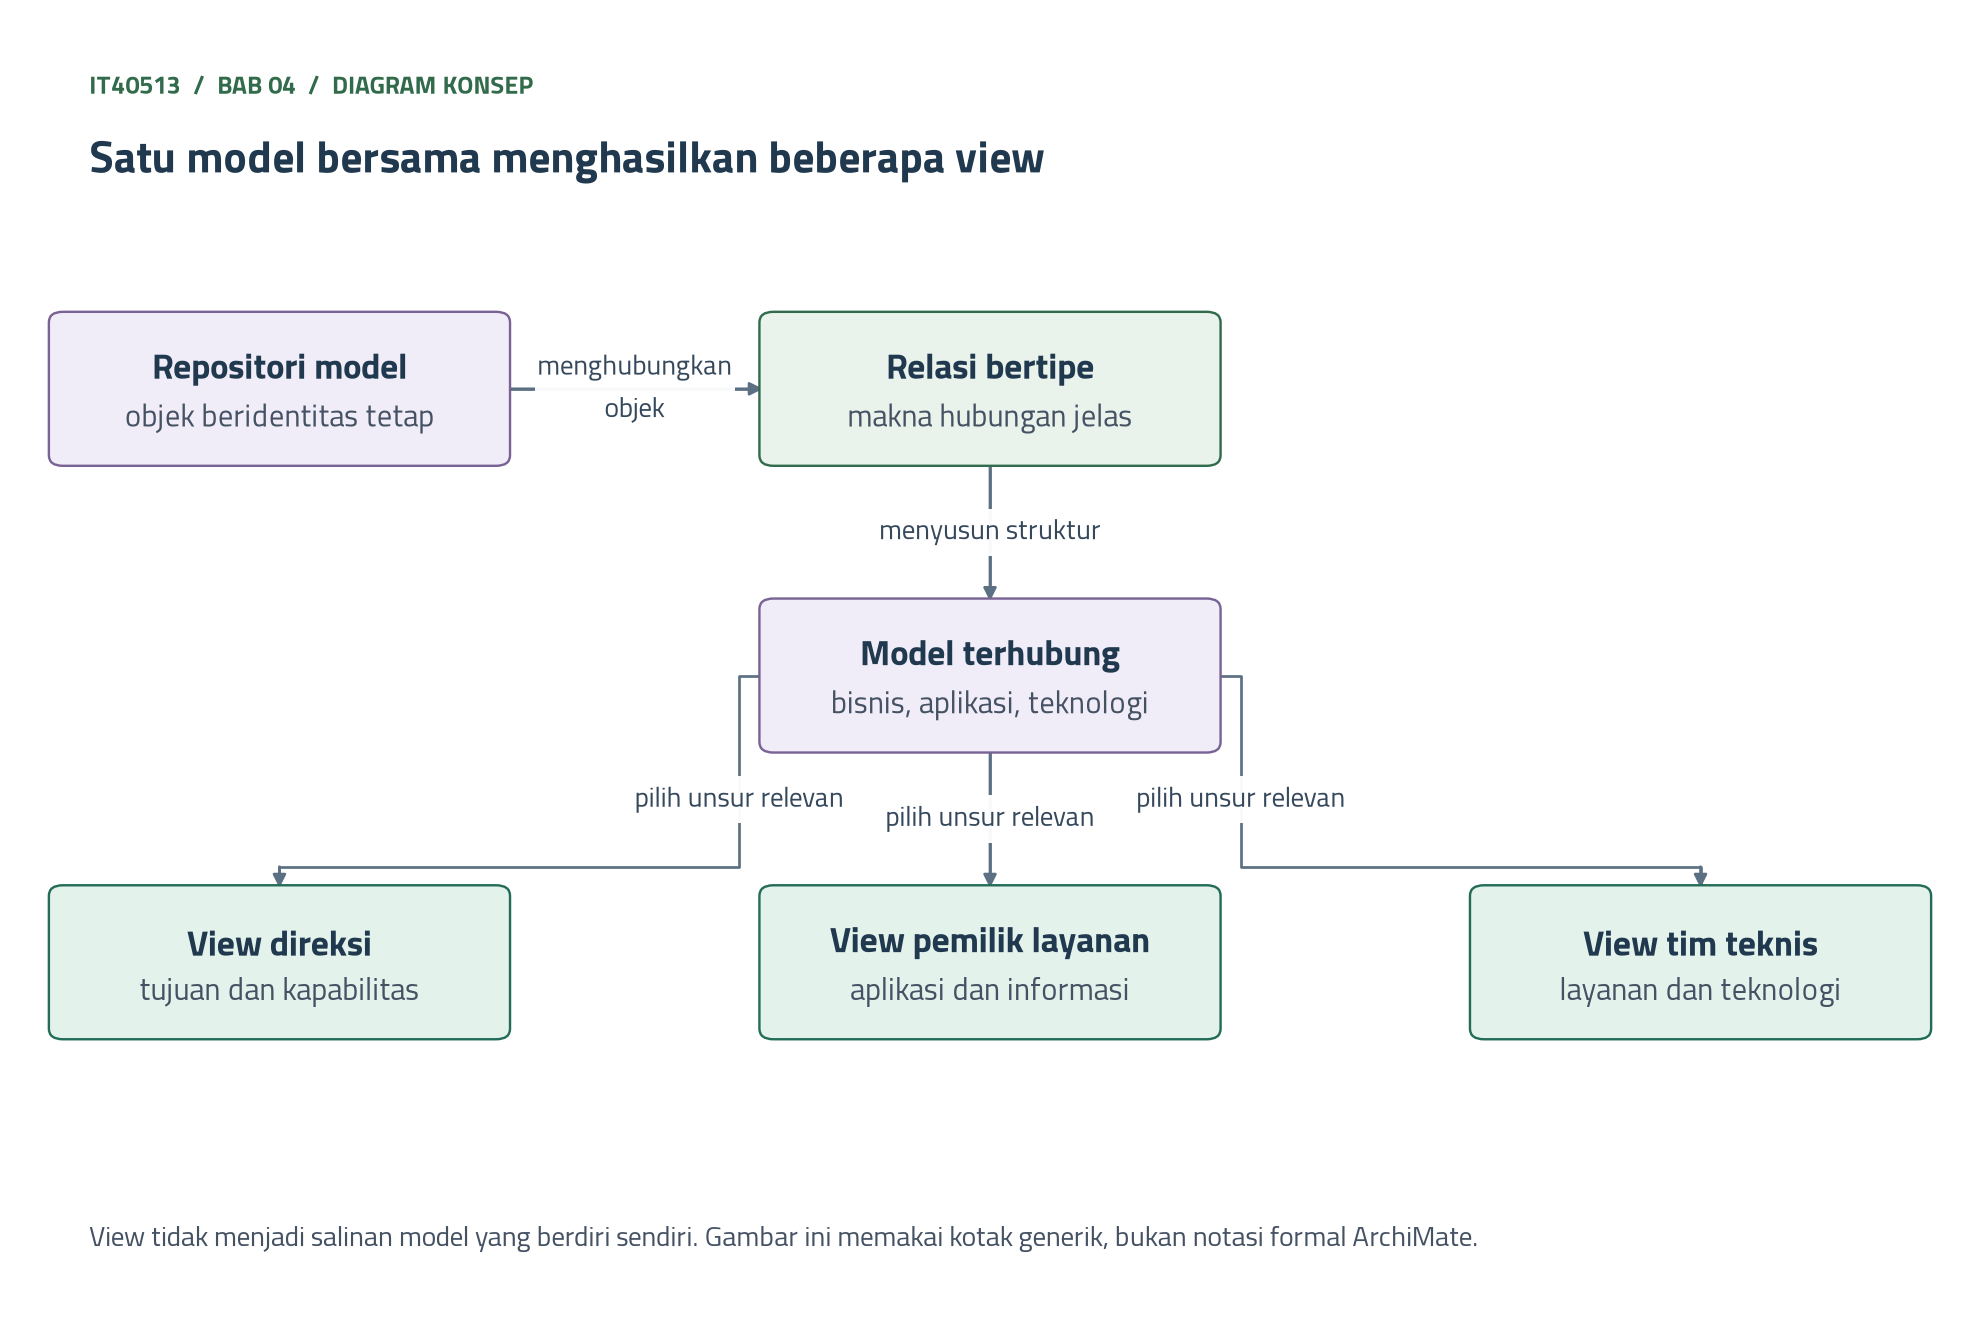
\includegraphics[width=\textwidth]{../figures/ch04-diagram-konsep.png}
  \caption{Satu model bersama menghasilkan beberapa view}
  \label{fig:ch04-ilustrasi}
\end{figure}

Tabel \ref{tab:ch04-viewpoint} memuat empat \textit{viewpoint} yang paling
sering dipakai di cetak biru \textit{capstone}.

\begin{table}[!htb]
  \centering
  \caption{Empat \textit{viewpoint} yang paling sering dipakai di cetak biru
           \textit{capstone}}
  \label{tab:ch04-viewpoint}
  \small
  \begin{tabularx}{\textwidth}{>{\raggedright\arraybackslash}p{2.3cm}>{\raggedright\arraybackslash}X>{\raggedright\arraybackslash}p{2.1cm}>{\raggedright\arraybackslash}X}
    \hline
    \textbf{\textit{Viewpoint}} & \textbf{Pertanyaan yang dijawab} & \textbf{Pembaca utama} & \textbf{Yang sengaja tidak tampil} \\
    \hline
    \textit{Layered} & Bagaimana satu layanan ditopang aplikasi dan teknologi dari ujung ke ujung? & Arsitek, kepala TI & Rantai motivasi, rincian langkah proses \\
    \hline
    \textit{Motivation} & Mengapa perubahan ini dilakukan, dan apa ukuran berhasilnya? & Direksi, pemilik program & Aplikasi dan teknologi \\
    \hline
    \textit{Application cooperation} & Aplikasi mana bertukar data dengan aplikasi mana? & Tim integrasi, analis teknologi & Proses bisnis, server \\
    \hline
    \textit{Capability map} & Apa saja yang mampu dilakukan organisasi? & Direksi, perencana strategi & Proses, aplikasi, unit organisasi \\
    \hline
  \end{tabularx}
\end{table}

Memilih \textit{viewpoint} dikerjakan dalam tiga langkah. Pertama,
\textit{concern} pembaca ditulis sebagai satu pertanyaan, misalnya ``aplikasi
mana yang menopang layanan janji temu?''. Kedua, dipilih
\textit{viewpoint} yang elemennya cukup untuk menjawab pertanyaan itu. Ketiga,
setiap elemen yang tidak membantu menjawab dibuang dari \textit{view}. Tim
\textit{capstone} memakai aturan praktis: bila sebuah \textit{view} memuat
lebih dari 20 elemen, \textit{view} itu dipecah atau pertanyaannya
dipersempit.

\begin{kasus}[title={Kasus Medikara Health: View untuk Direksi dan View untuk Tim TI}]
  Layanan janji temu yang sama dibahas di dua rapat. Rapat direksi bertanya
  aplikasi mana yang menopang layanan pasien dan di mana risikonya. Rapat tim
  TI bertanya bagaimana Medikara+ tersambung ke kelima SIMRS. Gambar
  \ref{fig:ch04-dua-view} memperlihatkan kedua \textit{view} itu, yang
  sama-sama diambil dari satu model.

  \textit{View} untuk direksi hanya memuat tiga layanan bisnis dan dua
  aplikasi. Kelima SIMRS diringkas menjadi satu kotak berwarna merah dengan
  keterangan ``5 versi berbeda'', karena yang perlu diketahui direksi adalah
  besarnya risiko, bukan nama tiap versi. Relasi melayani dari SIMRS ke
  layanan bisnis adalah relasi turunan, sehingga proses, fungsi, dan layanan
  aplikasi di antaranya boleh disembunyikan tanpa membuat \textit{view}
  menjadi salah.

  \textit{View} untuk tim TI membuang seluruh layanan bisnis, tetapi
  memecah SIMRS menjadi lima komponen aplikasi. Lima garis dari lima SIMRS ke
  Medikara+ langsung memperlihatkan lima integrasi \textit{point-to-point}
  yang harus dipelihara. Angka itu menjadi bahan perhitungan biaya integrasi
  di Bab 7.
\end{kasus}

\begin{figure}[!htb]
  \centering
  \begin{tikzpicture}[
  font=\scriptsize,
  elemen/.style={draw, rounded corners=1pt, minimum height=0.75cm, align=center,
                 font=\scriptsize\bfseries, fill=blue!8},
  kecil/.style={draw, rounded corners=1pt, minimum height=0.5cm, minimum width=2.3cm,
                align=center, font=\tiny\bfseries, fill=blue!8},
  panah/.style={-{Stealth[length=2mm]}, thick},
  layani/.style={-{Straight Barb[length=2mm, width=2.4mm]}, thick}
]
  % View untuk direksi: layanan pasien dan aplikasi pendukungnya saja.
  \node[font=\footnotesize\bfseries] at (2.45,3.1) {View untuk direksi};
  \node[elemen, minimum width=1.5cm] (s1) at (0.75,2.1)
    {Janji\\temu};
  \node[elemen, minimum width=1.5cm] (s2) at (2.45,2.1)
    {Pendaf-\\taran};
  \node[elemen, minimum width=1.5cm] (s3) at (4.15,2.1)
    {Telekon-\\sultasi};
  \node[elemen, fill=green!10, minimum width=2.0cm] (m) at (1.3,0.3)
    {Medikara+};
  \node[elemen, fill=red!22, minimum width=2.0cm] (s) at (3.6,0.3)
    {SIMRS\\{\tiny\mdseries 5 versi berbeda}};
  \draw[layani] (m) -- (s1);
  \draw[layani] (m) -- (s3);
  \draw[layani] (s) -- (s1);
  \draw[layani] (s) -- (s2);
  \node[font=\tiny, gray, align=center] at (2.45,-0.75)
    {\textit{concern}: aplikasi mana menopang layanan mana,\\dan di mana risikonya};

  \draw[gray, dashed] (5.35,3.4) -- (5.35,-2.3);

  % View untuk tim TI: integrasi dan infrastruktur di balik layanan yang sama.
  \node[font=\footnotesize\bfseries] at (8.75,3.1) {View untuk tim TI};
  \node[elemen, minimum width=2.1cm] (mk) at (6.75,1.0)
    {Medikara+\\{\tiny\mdseries komponen aplikasi}};
  \node[elemen, minimum width=2.1cm] (cloud) at (6.75,-0.65)
    {Server vendor\\{\tiny\mdseries \textit{node}, \textit{cloud}}};
  \node[kecil] (j) at (10.5,2.6) {SIMRS RS Jakarta};
  \node[kecil] (b) at (10.5,1.8) {SIMRS RS Bekasi};
  \node[kecil] (d) at (10.5,1.0) {SIMRS RS Depok};
  \node[kecil] (g) at (10.5,0.2) {SIMRS RS Bogor};
  \node[kecil] (n) at (10.5,-0.6) {SIMRS RS Bandung};
  \foreach \t in {j,b,d,g,n} {
    \draw[layani, red!60!black] (\t.west) -- (mk.east);
  }
  \draw[layani] (cloud) -- (mk);
  \node[font=\tiny, gray, align=center] at (8.75,-1.75)
    {\textit{concern}: lima integrasi \textit{point-to-point},\\tiap SIMRS di \textit{server} \textit{on-premise} sendiri};
\end{tikzpicture}

  \caption{Dua \textit{view} dari satu model: direksi melihat risiko pada
           layanan, tim TI melihat lima integrasi \textit{point-to-point}}
  \label{fig:ch04-dua-view}
\end{figure}

Dua hal pada \textit{view} sering tertukar. Pembagiannya begini.
Menyembunyikan elemen di sebuah \textit{view} adalah keputusan penyajian,
sedangkan menghapus elemen dari model adalah keputusan isi. \textit{View}
direksi yang hanya memuat lima elemen tidak berarti model Medikara hanya
berisi lima elemen. Karena itu setiap \textit{view} sebaiknya diberi catatan
singkat tentang pertanyaan yang dijawabnya, agar pembaca tahu bahwa yang
tidak tampil memang sengaja tidak ditampilkan.

\section{Bekerja dengan Archi}

Archi adalah alat pemodelan ArchiMate yang gratis dan bersumber terbuka.
Versi 5.10.0 dirilis 3 September 2026, mendukung ArchiMate 3.2, dan tersedia
untuk Windows 10 atau lebih baru (64-bit), macOS 11 atau lebih baru (Apple
Silicon dan Intel), serta distribusi Linux 64-bit \cite{archi}. Langkah
pemasangannya ditulis di \berkas{sources/chapter04/panduan-instalasi-archi.md}.
Satu berkas model Archi berekstensi \texttt{.archimate} menyimpan seluruh
elemen, relasi, dan \textit{view}, sehingga berkas itu dapat diperlakukan
sebagai repositori kecil milik tim.

Pohon model Archi selalu dimulai dengan folder tetap: Strategy, Business,
Application, Technology \& Physical, Motivation, Implementation \& Migration,
Other, Relations, dan Views. Elemen hanya dapat disimpan di folder yang
sesuai dengan jenisnya. Komponen aplikasi, misalnya, tidak dapat dipindah ke
folder Business. Tim boleh membuat subfolder di dalam tiap folder tetap,
misalnya subfolder per rumah sakit di dalam folder Application, asalkan
polanya disepakati di awal.

Konvensi penamaan menentukan apakah model masih dapat dibaca setelah tiga
bulan dan empat penulis. Tabel \ref{tab:ch04-konvensi} memuat konvensi yang
dipakai tim \textit{capstone}. Versi lengkapnya ada di
\berkas{sources/chapter04/konvensi-penamaan-model.md}.

\begin{table}[!htb]
  \centering
  \caption{Konvensi penamaan elemen untuk model tim \textit{capstone}}
  \label{tab:ch04-konvensi}
  \small
  \begin{tabularx}{\textwidth}{>{\raggedright\arraybackslash}p{2.4cm}>{\raggedright\arraybackslash}X>{\raggedright\arraybackslash}p{3.1cm}>{\raggedright\arraybackslash}p{2.6cm}}
    \hline
    \textbf{Jenis elemen} & \textbf{Pola nama} & \textbf{Contoh benar} & \textbf{Dihindari} \\
    \hline
    Proses & Kata kerja dan objeknya & Membuat Janji Temu & Proses Janji Temu \\
    \hline
    Fungsi & Kata benda berimbuhan pe-an & Pengelolaan Jadwal Dokter & Kelola Jadwal \\
    \hline
    Layanan & Kata ``Layanan'' dan hasil yang diterima pemakai & Layanan Pemesanan Jadwal & API Jadwal v2 \\
    \hline
    Komponen aplikasi & Nama yang dipakai pengguna, ditambah lokasi bila versinya berbeda & SIMRS RS Jakarta & HIS Bekasi \\
    \hline
    Peran & Nama peran, bukan nama orang & Petugas Pendaftaran & Bu Rina \\
    \hline
    Objek data & Kata benda tunggal dalam bahasa bisnis & Data Jadwal Dokter & tbl\_jadwal \\
    \hline
    \textit{View} & Jenis \textit{view}, titik dua, dan topiknya & Layered View: Janji Temu Rawat Jalan & Default View \\
    \hline
  \end{tabularx}
\end{table}

Nama saja belum cukup. Setiap elemen penting diberi properti, yaitu pasangan
kunci dan nilai yang tersimpan bersama elemen. Tim \textit{capstone} memakai
empat properti: Pemilik, Status (saat ini, target, atau dihentikan), Sumber
(asal informasinya, misalnya wawancara atau katalog aset), dan Lokasi untuk
\textit{node}. Properti Pemilik pada komponen aplikasi wajib diisi sejak
sekarang, karena katalog aplikasi di Bab 7 disusun langsung dari properti
itu. Kolom dokumentasi dipakai untuk satu atau dua kalimat penjelasan dalam
bahasa bisnis.

Archi menyediakan beberapa cara untuk membagikan model kepada pembaca yang
tidak memasang Archi. \textit{View} dapat diekspor sebagai berkas gambar untuk
dokumen dan slide. Seluruh model dapat diekspor sebagai laporan HyperText
Markup Language (HTML), yaitu situs kecil yang dapat dibuka di peramban dan
ditelusuri per elemen. Model juga dapat diekspor ke berkas Comma-Separated
Values (CSV) untuk diolah di \textit{spreadsheet}, atau ke Open Exchange
Format untuk dipindahkan ke alat pemodelan lain. Sebelum dibagikan, model
diperiksa dengan fitur Validator di Archi, yang menandai antara lain elemen
yang tidak dipakai di \textit{view} mana pun dan elemen yang mungkin ganda.

Pertanyaan kemudian muncul: bagaimana empat anggota tim bekerja di satu
model? Ada dua pilihan. Pilihan pertama, pemodel memegang berkas induk, dan
anggota lain mengirim perubahan yang kemudian dimasukkan pemodel. Cara ini
sederhana dan cocok untuk tim kecil, tetapi pemodel menjadi titik antrean.
Pilihan kedua memakai \textit{plug-in} coArchi, yang menyimpan model di
repositori Git sehingga tiap anggota dapat menyimpan perubahan lalu
menggabungkannya, dengan dialog bantuan bila terjadi konflik. Versi 0.9.8
dapat diunduh gratis dan membutuhkan repositori Git di sebuah server Git
\cite{c04-archiplugin}. Keputusan ini punya dua konsekuensi. Pertama, pilihan
pertama tidak membutuhkan keterampilan baru, tetapi riwayat perubahan hanya
tercatat bila pemodel rajin menyimpan salinan bertanggal. Kedua, pilihan
kedua mencatat riwayat secara otomatis, tetapi setiap anggota harus belajar
dasar Git.

\begin{pendalaman}[title={Pendalaman Teknis (opsional): Memeriksa Model secara Otomatis}]
  Validator Archi memeriksa aturan bahasa, tetapi tidak mengenal konvensi
  tim. Pemeriksaan konvensi dapat diotomatiskan dengan dua cara.

  Cara pertama memakai jArchi, \textit{plug-in} yang menambahkan bahasa skrip
  JavaScript ke dalam Archi. Skrip jArchi dapat membaca dan mengubah seluruh
  isi model, misalnya untuk membuat laporan, mewarnai \textit{heatmap},
  mengimpor data, atau memproses banyak elemen sekaligus. Kode sumbernya
  gratis di GitHub, sedangkan versi siap pasang disediakan bagi pendukung
  proyek Archi. Versi 1.12 membutuhkan Archi 5.8 atau lebih baru
  \cite{c04-archiplugin}.

  Cara kedua bekerja di luar Archi lewat Open Exchange Format, yaitu format
  berbasis Extensible Markup Language (XML) yang distandarkan The Open Group
  untuk memindahkan model antaralat \cite{c04-exchange}. Format ini terdiri
  atas tiga skema, yaitu model, \textit{view}, dan diagram, dan berlaku untuk
  ArchiMate 3.1 dan 3.2. Tujuannya pertukaran, bukan penyimpanan tetap,
  sehingga berkas kerja sehari-hari tetap berkas \texttt{.archimate}.

  Skrip \texttt{periksa-model.py} membaca kedua format itu, lalu memeriksa
  referensi relasi yang putus, elemen yang tidak tampil di \textit{view} atau
  tidak punya relasi, nama bawaan Archi yang belum diganti, awalan nama
  menurut Tabel \ref{tab:ch04-konvensi}, dan properti Pemilik pada komponen
  aplikasi. Listing \ref{lst:ch04-periksa} memperlihatkan salah satu
  pemeriksaannya.

\begin{lstlisting}[language=Python, basicstyle=\ttfamily\scriptsize,
  keywordstyle=\color{blue}\bfseries, commentstyle=\color{gray}\itshape,
  stringstyle=\color{red}, numbers=left, numberstyle=\tiny\color{gray},
  frame=lines, backgroundcolor=\color{lightgray!10}, breaklines=true,
  showstringspaces=false, tabsize=2,
  caption={Mencari elemen yang tidak tampil atau tidak punya relasi, tersedia di \berkas{sources/chapter04/periksa-model.py}},
  label={lst:ch04-periksa}]
def periksa_pemakaian_elemen(daftar_elemen, daftar_relasi, id_elemen_tampil):
  """Mencari elemen yang tidak tampil di view atau tidak punya relasi."""
  id_terhubung = set()
  for relasi in daftar_relasi:
    id_terhubung.add(relasi["sumber"])
    id_terhubung.add(relasi["tujuan"])
  peringatan = []
  for elemen in daftar_elemen:
    if elemen["jenis"] in JENIS_TANPA_ATURAN_NAMA:
      continue
    if elemen["id"] not in id_elemen_tampil:
      peringatan.append(f"Belum tampil di view mana pun: {elemen['nama']}")
    if elemen["id"] not in id_terhubung:
      peringatan.append(f"Tidak punya relasi: {elemen['nama']}")
  return peringatan
\end{lstlisting}

  Pada model contoh Medikara, skrip melaporkan 26 elemen, 30 relasi, nol
  kesalahan, dan nol peringatan. Listing \ref{lst:ch04-periksa-jalan} memuat
  hasilnya pada salinan model contoh dalam Open Exchange Format yang sengaja
  ditambah dua cacat: satu komponen aplikasi bernama bawaan tanpa relasi, dan
  satu proses yang relasinya menunjuk elemen yang tidak ada.

\begin{lstlisting}[language=bash,
  caption={Keluaran pemeriksa pada model yang sengaja diberi cacat, memakai \berkas{sources/chapter04/periksa-model.py}},
  label={lst:ch04-periksa-jalan}]
python periksa-model.py medikara-cacat.xml

# Keluarannya (ringkasan jenis elemen dipotong):
# Format: Open Exchange Format
# Elemen: 28, relasi: 31, elemen yang tampil di view: 26
# Kesalahan: 1
#   - Relasi id-rbaru (Serving): tujuan 'id-hilang' tidak ditemukan
# Peringatan: 6
#   - Belum tampil di view mana pun: Application Component
#   - Tidak punya relasi: Application Component
#   - Belum tampil di view mana pun: Pendaftaran Pasien
#   - Nama bawaan Archi belum diganti: Application Component
#   - Proses sebaiknya diawali kata kerja: Pendaftaran Pasien
#   - Properti 'Pemilik' kosong: Application Component
\end{lstlisting}

  Skrip keluar dengan status 1 bila ada kesalahan, sehingga pemeriksaan ini
  dapat dipasang sebagai langkah otomatis sebelum model induk diperbarui.
  Peringatan tidak menggagalkan pemeriksaan, karena peringatan sering hanya
  menandai pekerjaan yang belum selesai.
\end{pendalaman}

\section{ArchiMate 4 dan Dampaknya bagi Pemodel}

The Open Group menerbitkan ArchiMate 4 (dokumen C260) pada 27 April 2026
sebagai pengganti ArchiMate 3.2 \cite{archimate4}. Pengumumannya menekankan
kesesuaian yang kuat di tingkat pengguna, sehingga pemodel dapat berpindah
tanpa gangguan besar \cite{archimate4}. Perubahannya tetap terasa.
Istilah lapisan diganti domain. Elemen perilaku yang dulu terpisah per
lapisan digabung menjadi satu set layanan, proses, fungsi, dan peristiwa.
Peran bisnis diganti peran umum yang dapat ditugaskan kepada elemen
struktur aktif internal mana pun. Kolaborasi bisnis, aplikasi, dan teknologi
digabung menjadi satu elemen kolaborasi. Relasi dapat diberi multiplisitas,
yaitu batas jumlah elemen di tiap ujungnya. Beberapa elemen dihapus: interaksi
bisnis, interaksi aplikasi, interaksi teknologi, \textit{constraint},
kontrak, \textit{gap}, dan representasi \cite{archimate4}. Tabel
\ref{tab:ch04-archimate4} merangkum perubahan yang paling terasa bagi model
\textit{capstone}.

\begin{table}[!htb]
  \centering
  \caption{Perubahan utama dari ArchiMate 3.2 ke ArchiMate 4 dan dampaknya
           pada model Medikara}
  \label{tab:ch04-archimate4}
  \small
  \begin{tabularx}{\textwidth}{>{\raggedright\arraybackslash}p{3.0cm}>{\raggedright\arraybackslash}p{3.6cm}X}
    \hline
    \textbf{ArchiMate 3.2} & \textbf{ArchiMate 4} & \textbf{Dampak pada model Medikara} \\
    \hline
    Lapisan bisnis, aplikasi, teknologi & Domain & Istilah berubah, susunan \textit{view} tetap \\
    \hline
    Proses, fungsi, layanan, dan peristiwa per lapisan & Satu set elemen perilaku umum & Layanan bisnis dan layanan aplikasi menjadi satu jenis \\
    \hline
    Peran bisnis & Peran umum & Peran dapat dipasang pada komponen aplikasi atau \textit{node} \\
    \hline
    Kolaborasi per lapisan & Satu elemen kolaborasi & Kolaborasi antarrumah sakit dan antaraplikasi memakai elemen yang sama \\
    \hline
    Relasi tanpa jumlah & Relasi dengan multiplisitas & ``Satu pasien punya banyak janji temu'' dapat dinyatakan di model \\
    \hline
    Interaksi, \textit{constraint}, kontrak, \textit{gap}, representasi & Dihapus & Elemen \textit{gap} yang dipakai di Bab 11 perlu dicatat dengan cara lain \\
    \hline
  \end{tabularx}
\end{table}

Pertanyaan kemudian muncul: mengapa mata kuliah ini tetap memakai ArchiMate
3.2? Alasannya tiga. Pertama, Archi 5.10.0 masih mendukung ArchiMate 3.2 dan
belum mendukung ArchiMate 4 \cite{archi}. Kedua, Open Exchange Format yang
berlaku saat ini disusun untuk ArchiMate 3.1 dan 3.2 \cite{c04-exchange},
sehingga model tim masih dapat dipindahkan ke alat lain. Ketiga, cetak biru
\textit{capstone} dikerjakan selama satu semester, dan berganti versi bahasa di
tengah jalan menambah risiko tanpa menambah nilai bagi pembaca cetak biru.

Keputusan ini punya dua konsekuensi. Pertama, model tim akan perlu
dipindahkan suatu hari, ketika alatnya sudah mendukung ArchiMate 4. Kedua,
pemindahan itu dapat dibuat murah bila model disiapkan sejak sekarang. Empat
kebiasaan berikut membantu:

\begin{enumerate}
  \item Interaksi tidak dipakai. Kerja sama beberapa pihak dimodelkan sebagai
        proses dengan beberapa elemen struktur aktif yang ditugaskan
        kepadanya, sesuai arah ArchiMate 4.
  \item \textit{Constraint} diganti \textit{requirement} yang diberi properti
        Jenis bernilai ``batasan'', dan kontrak diganti objek bisnis yang
        diberi properti serupa. Artinya tidak hilang ketika jenis elemennya
        dihapus.
  \item Setiap layanan dan proses diberi nama yang menyiratkan domainnya,
        misalnya Layanan Pemesanan Jadwal untuk layanan aplikasi. Ketika
        jenis elemennya digabung, nama tetap membedakan keduanya.
  \item Jumlah yang penting ditulis di dokumentasi relasi, misalnya ``satu
        dokter punya banyak slot jadwal''. Catatan itu kelak dipindah menjadi
        multiplisitas.
\end{enumerate}

\section{Aktivitas: Memodelkan Satu Layanan dari Pasien sampai Server}

Aktivitas ini menghasilkan model berlapis pertama milik tim. Model itu
menjadi fondasi repositori yang terus diisi sampai akhir semester: Bab 5
menambahkan kapabilitas dan \textit{value stream}, Bab 6 menambahkan objek
data, dan Bab 7 menambahkan katalog aplikasi dan teknologi. Tim yang memakai
organisasi sendiri memodelkan satu layanan inti organisasinya. Tim yang
memakai Medikara Health memodelkan layanan janji temu rawat jalan atau layanan
lain yang setara, misalnya pendaftaran pasien atau pengambilan hasil
laboratorium.

\textbf{Pembagian peran.}

\begin{itemize}
  \item \textbf{Analis bisnis} memodelkan lapisan bisnis: pelaku, peran,
        layanan bisnis, proses, dan objek bisnis.
  \item \textbf{Analis teknologi} memodelkan lapisan aplikasi dan teknologi:
        komponen aplikasi, layanan aplikasi, objek data, \textit{node}, dan
        layanan teknologi. Kedua analis bekerja berpasangan dan menyepakati
        titik sambung di antara lapisan mereka.
  \item \textbf{Pemodel} menyiapkan berkas model bersama, struktur folder,
        konvensi penamaan, dan cara kerja bersama, lalu menjaga agar seluruh
        elemen mengikuti konvensi itu.
  \item \textbf{Koordinator} memastikan rantai motivasi dari C1 ikut
        dimodelkan, lalu memeriksa silang istilah dengan glosarium bersama.
\end{itemize}

\textbf{Langkah kerja.}

\begin{enumerate}
  \item Setiap anggota memasang Archi 5.10.0 mengikuti
        \berkas{sources/chapter04/panduan-instalasi-archi.md}, lalu membuka
        \berkas{sources/chapter04/medikara-janji-temu.archimate} untuk
        melihat contoh model yang sudah jadi.
  \item Pemodel membuat berkas model tim, menyiapkan subfolder, dan
        menetapkan konvensi penamaan berdasarkan
        \berkas{sources/chapter04/konvensi-penamaan-model.md}. Tim memilih
        satu dari dua cara kerja bersama yang dibahas di subbab Archi.
  \item Tim memilih satu layanan inti, lalu menulis batasnya dalam satu
        kalimat di \berkas{sources/chapter04/lembar-kerja-model-berlapis.md}:
        siapa penerimanya, apa hasilnya, dan di fasilitas mana layanan itu
        berjalan.
  \item Analis bisnis dan analis teknologi mengisi daftar elemen tiap lapisan
        di lembar kerja, lalu memasukkannya ke Archi sesuai konvensi.
  \item Keduanya menyepakati titik sambung: layanan aplikasi mana yang
        melayani proses bisnis, dan layanan teknologi mana yang melayani
        komponen aplikasi.
  \item Pemodel menghubungkan elemen dengan relasi yang tepat menurut Tabel
        \ref{tab:ch04-relasi}, lalu menyusun \textit{layered view}.
  \item Koordinator memindahkan rantai motivasi C1, dari \textit{driver}
        sampai \textit{requirement}, ke \textit{motivation view}, lalu
        menghubungkan minimal satu \textit{requirement} ke elemen inti yang
        mewujudkannya.
  \item Tim memeriksa silang setiap nama elemen dengan glosarium C1,
        menjalankan Validator Archi, lalu mengekspor laporan HTML sebagai
        lampiran C2.
\end{enumerate}

\textbf{Luaran dan kaitan dengan \textit{capstone}.} Luarannya berupa berkas
model ArchiMate awal yang memuat minimal satu \textit{layered view} dan satu
\textit{motivation view}, beserta laporan HTML-nya. Luaran ini menjadi
fondasi tonggak C2 Kondisi Saat Ini. Artefak Pertemuan 5 sampai 7 dimasukkan
ke model yang sama, sehingga dokumen C2 yang ditinjau menjelang UTS tidak
berisi gambar yang saling bertentangan.

\textbf{Kriteria penilaian.} Tabel \ref{tab:ch04-kriteria} memuat kriteria
yang dipakai saat model ditinjau pada tatap muka hari Sabtu.

\begin{table}[!htb]
  \centering
  \caption{Kriteria penilaian model berlapis awal}
  \label{tab:ch04-kriteria}
  \small
  \begin{tabularx}{\textwidth}{>{\raggedright\arraybackslash}p{3.6cm}rX}
    \hline
    \textbf{Kriteria} & \textbf{Bobot} & \textbf{Tanda terpenuhi} \\
    \hline
    Kelengkapan rantai & 30\% & Rantai tidak putus dari penerima layanan sampai \textit{node} \\
    \hline
    Ketepatan relasi & 25\% & Arah melayani benar, asosiasi hanya dipakai bila tidak ada relasi lain yang cocok \\
    \hline
    Keterbacaan \textit{view} & 20\% & Paling banyak 20 elemen per \textit{view}, tata letak per lapisan \\
    \hline
    Keterlacakan ke C1 & 15\% & Minimal satu \textit{requirement} terhubung ke elemen inti \\
    \hline
    Konsistensi nama & 10\% & Nama sama dengan glosarium C1 dan mengikuti konvensi \\
    \hline
  \end{tabularx}
\end{table}

\textbf{Berkas pendukung.} Seluruh berkas tersedia di
\berkas{sources/chapter04/}: panduan pemasangan Archi, konvensi penamaan dan
daftar periksa model, lembar kerja model berlapis, contoh model Medikara, dan
skrip pemeriksa model.

\textbf{Etika.} Model organisasi nyata hanya dibuat seizin organisasinya,
dan nama sistem yang sensitif boleh disamarkan. Model tidak memuat data
pribadi. Elemen peran ditulis sebagai nama peran, bukan nama karyawan, dan
contoh data pasien tidak pernah dimasukkan ke dokumentasi elemen.

\textbf{Pendalaman teknis (opsional).} Mahasiswa berlatar CS, SE, atau TI
dapat mengekspor model tim ke Open Exchange Format, menjalankan
\texttt{periksa-model.py} pada berkas hasil ekspor, lalu membandingkan
temuannya dengan temuan Validator Archi. Perbedaan keduanya menunjukkan
aturan mana yang hanya berasal dari konvensi tim.

\section{Ringkasan}

Gambar kotak dan panah gagal sebagai alat komunikasi arsitektur karena
artinya disimpan di kepala pembuatnya. Model menyimpan arti itu di elemen dan
relasi yang punya definisi baku, sedangkan \textit{view} hanya menampilkan
sebagian isi model untuk pembaca tertentu. Satu elemen dibuat sekali di
repositori dan dipakai di banyak \textit{view}, sehingga perubahan cukup
dikerjakan sekali. Pada contoh Medikara, satu sistem yang muncul di 14
gambar dengan empat nama berbeda menjadi satu elemen dengan satu nama.

Kerangka inti ArchiMate 3.2 berupa kisi tiga lapisan, yaitu bisnis,
aplikasi, dan teknologi, kali tiga aspek, yaitu struktur aktif, perilaku, dan
struktur pasif. Pola itu sama dengan kalimat sederhana: subjek, predikat, dan
objek. Lapisan disambung lewat layanan, dan di sekeliling kisi inti terdapat
elemen strategi, motivasi, serta implementasi dan migrasi yang dipakai di
bab-bab berikutnya.

Relasi memberi arti pada garis. Relasi struktural menyatakan susunan, relasi
dependensi menyatakan ketergantungan, dan relasi dinamis menyatakan urutan dan
perpindahan. Archi menolak relasi yang tidak sah, tetapi tidak dapat menolak
relasi yang sah namun keliru artinya, seperti arah melayani yang terbalik atau
asosiasi yang dipakai untuk segala hal. Aturan penurunan memungkinkan rantai
panjang diringkas menjadi satu relasi tanpa membuat \textit{view} menjadi
salah.

\textit{Viewpoint} menentukan apa yang boleh tampil untuk menjawab satu
\textit{concern}. Layanan janji temu Medikara yang sama menghasilkan
\textit{view} lima elemen untuk direksi dan \textit{view} lima integrasi
\textit{point-to-point} untuk tim TI. Archi menyediakan folder tetap,
properti, Validator, laporan HTML, dan Open Exchange Format, sedangkan
konvensi penamaan dan cara kerja bersama tetap harus disepakati tim.

ArchiMate 4 menggabungkan elemen perilaku lintas lapisan, menyediakan peran
umum dan multiplisitas relasi, serta menghapus beberapa elemen. Mata kuliah
ini tetap memakai ArchiMate 3.2 karena Archi belum mendukung versi baru,
tetapi model disiapkan agar mudah dipindahkan. Pesan utama bab ini: cetak biru
yang dapat dipercaya dibangun dari satu model bersama, bukan dari kumpulan
gambar, dan setiap gambar di dalamnya adalah jawaban atas pertanyaan seorang
pembaca tertentu.

\section{Latihan}

Seluruh berkas yang dipakai pada latihan ini tersedia di
\berkas{sources/chapter04/}. Latihan membutuhkan Archi 5.10.0 dan model contoh
\berkas{sources/chapter04/medikara-janji-temu.archimate}. Lembar isian yang
sama juga tersedia dalam
\berkas{sources/chapter04/lembar-kerja-model-berlapis.md}. Hasil tiap
mahasiswa boleh berbeda, karena satu layanan dapat dimodelkan dengan beberapa
cara yang sama-sama sah. Yang dinilai adalah alasan di balik setiap pilihan
elemen dan relasi.

\subsection*{Latihan 1: Rantai Elemen untuk Layanan Pendaftaran}

Latihan ini membuktikan bahwa satu layanan dapat ditelusuri tanpa putus dari
pasien sampai server, dan bahwa setiap sambungan dapat dibaca sebagai
kalimat yang bermakna.

\begin{enumerate}
  \item Tentukan layanan bisnis pendaftaran pasien rawat jalan dan aktor yang
        dilayaninya.
  \item Turun ke proses bisnis yang mewujudkan layanan itu, beserta peran yang
        ditugaskan padanya.
  \item Cari layanan aplikasi yang melayani proses itu, lalu komponen
        aplikasi yang mewujudkannya. Untuk Medikara, komponennya adalah SIMRS.
  \item Lanjutkan ke layanan teknologi dan \textit{node}, sampai ke
        server basis data SIMRS.
  \item Tulis setiap langkah ke Tabel \ref{tab:ch04-lat1-hasil}, lengkap
        dengan jenis elemen dan jenis relasinya. Tabel
        \ref{tab:ch04-lat1-contoh} memperlihatkan contoh terisi untuk
        layanan janji temu, diambil dari model contoh.
  \item Jawab tiga pertanyaan berikut. Pertama, berapa langkah rantai
        pendaftaran dibandingkan dengan sembilan langkah rantai janji temu,
        dan apa arti selisihnya? Kedua, bila SIMRS RS Jakarta diganti,
        layanan bisnis mana saja yang ikut terdampak menurut rantai yang
        disusun? Ketiga, langkah mana yang paling sulit ditentukan
        relasinya, dan mengapa?
\end{enumerate}

\begin{table}[!htb]
  \centering
  \caption{Contoh hasil Latihan 1 yang sudah terisi: rantai layanan janji
           temu menurut model contoh Medikara}
  \label{tab:ch04-lat1-contoh}
  \small
  \begin{tabularx}{\textwidth}{c>{\raggedright\arraybackslash}X>{\raggedright\arraybackslash}p{1.7cm}>{\raggedright\arraybackslash}X}
    \hline
    \textbf{No.} & \textbf{Sumber (jenis)} & \textbf{Relasi} & \textbf{Tujuan (jenis)} \\
    \hline
    1 & Layanan Janji Temu Rawat Jalan (layanan bisnis) & melayani & Pasien (aktor bisnis) \\
    \hline
    2 & Membuat Janji Temu (proses bisnis) & realisasi & Layanan Janji Temu Rawat Jalan \\
    \hline
    3 & Layanan Pemesanan Jadwal (layanan aplikasi) & melayani & Membuat Janji Temu \\
    \hline
    4 & Medikara+ (komponen aplikasi) & realisasi & Layanan Pemesanan Jadwal \\
    \hline
    5 & Layanan Jadwal Dokter (layanan aplikasi) & melayani & Medikara+ \\
    \hline
    6 & Pengelolaan Jadwal Dokter (fungsi aplikasi) & realisasi & Layanan Jadwal Dokter \\
    \hline
    7 & SIMRS RS Jakarta (komponen aplikasi) & penugasan & Pengelolaan Jadwal Dokter \\
    \hline
    8 & Layanan Basis Data (layanan teknologi) & melayani & SIMRS RS Jakarta \\
    \hline
    9 & Server Basis Data SIMRS (\textit{node}) & realisasi & Layanan Basis Data \\
    \hline
  \end{tabularx}
\end{table}

\begin{table}[!htb]
  \centering
  \caption{Lembar isian Latihan 1: rantai layanan pendaftaran}
  \label{tab:ch04-lat1-hasil}
  \small
  \begin{tabularx}{\textwidth}{c>{\raggedright\arraybackslash}X>{\raggedright\arraybackslash}p{1.7cm}>{\raggedright\arraybackslash}X}
    \hline
    \textbf{No.} & \textbf{Sumber (jenis)} & \textbf{Relasi} & \textbf{Tujuan (jenis)} \\
    \hline
    1 & \dots & \dots & Pasien (aktor bisnis) \\
    \hline
    2 & \dots & \dots & \dots \\
    \hline
    3 & \dots & \dots & \dots \\
    \hline
    4 & \dots & \dots & \dots \\
    \hline
    5 & \dots & \dots & \dots \\
    \hline
    6 & \dots & \dots & \dots \\
    \hline
    7 & Server basis data SIMRS (\textit{node}) & \dots & \dots \\
    \hline
  \end{tabularx}
\end{table}

\subsection*{Latihan 2: Memilih Viewpoint untuk Direktur}

Latihan ini membuktikan bahwa \textit{view} yang baik ditentukan oleh
pertanyaan pembacanya, bukan oleh banyaknya isi model.

\begin{enumerate}
  \item Tulis \textit{concern} direktur sebagai satu pertanyaan: aplikasi mana
        yang mendukung tiap layanan pasien?
  \item Daftar jenis elemen yang dibutuhkan untuk menjawab pertanyaan itu, dan
        jenis elemen yang tidak dibutuhkan.
  \item Pilih \textit{viewpoint} ArchiMate 3.2 yang paling cocok. Gunakan
        Tabel \ref{tab:ch04-viewpoint} sebagai titik awal, lalu periksa daftar
        \textit{viewpoint} di menu properti \textit{view} di Archi.
  \item Buat \textit{view} itu di Archi dari elemen model contoh, lalu hitung
        jumlah elemen yang tampil dibandingkan dengan 16 elemen pada
        \textit{layered view} model contoh.
  \item Isi Tabel \ref{tab:ch04-lat2-hasil}. Tabel \ref{tab:ch04-lat2-contoh}
        memperlihatkan contoh terisi untuk pembaca dan \textit{concern} yang
        berbeda.
  \item Jawab tiga pertanyaan berikut. Pertama, berapa persen elemen
        \textit{layered view} yang tetap tampil di \textit{view} direktur?
        Kedua, relasi turunan mana yang dipakai agar \textit{view} tetap benar
        walaupun elemen perantaranya disembunyikan? Ketiga, apa akibatnya bila
        \textit{view} direktur juga menampilkan server?
\end{enumerate}

\begin{table}[!htb]
  \centering
  \caption{Contoh hasil Latihan 2 yang sudah terisi untuk kepala Divisi
           Teknologi Informasi}
  \label{tab:ch04-lat2-contoh}
  \small
  \begin{tabularx}{\textwidth}{>{\raggedright\arraybackslash}p{3.2cm}X}
    \hline
    \textbf{Aspek} & \textbf{Isian} \\
    \hline
    Pembaca & Kepala Divisi Teknologi Informasi \\
    \hline
    \textit{Concern} & Server mana yang menopang tiap aplikasi? \\
    \hline
    \textit{Viewpoint} & \textit{Technology usage} \\
    \hline
    Elemen yang tampil & 2 komponen aplikasi, 2 \textit{node}, 1 perangkat lunak sistem, 1 layanan teknologi \\
    \hline
    Elemen yang disembunyikan & Aktor, proses, layanan bisnis, objek bisnis, seluruh elemen motivasi \\
    \hline
    Jumlah elemen & 6 dari 16 elemen \textit{layered view}, atau 38 persen \\
    \hline
    Alasan & Pertanyaannya tentang ketergantungan aplikasi pada server, bukan tentang layanan pasien \\
    \hline
  \end{tabularx}
\end{table}

\begin{table}[!htb]
  \centering
  \caption{Lembar isian Latihan 2 untuk direktur}
  \label{tab:ch04-lat2-hasil}
  \small
  \begin{tabularx}{\textwidth}{>{\raggedright\arraybackslash}p{3.2cm}X}
    \hline
    \textbf{Aspek} & \textbf{Isian} \\
    \hline
    Pembaca & Direktur \\
    \hline
    \textit{Concern} & Aplikasi mana yang mendukung tiap layanan pasien? \\
    \hline
    \textit{Viewpoint} & \dots \\
    \hline
    Elemen yang tampil & \dots \\
    \hline
    Elemen yang disembunyikan & \dots \\
    \hline
    Jumlah elemen & \dots{} dari 16 elemen \textit{layered view}, atau \dots{} persen \\
    \hline
    Alasan & \dots \\
    \hline
  \end{tabularx}
\end{table}

\subsection*{Latihan 3: Menghitung Dampak ArchiMate 4}

Latihan ini membuktikan bahwa dampak sebuah versi standar baru dapat dihitung
dari isi model, bukan sekadar diperkirakan.

\begin{enumerate}
  \item Buka model contoh Medikara atau model tim, lalu hitung jumlah elemen
        per jenis. Jumlah itu terlihat di pohon model Archi, atau di
        ringkasan keluaran \texttt{periksa-model.py}.
  \item Tandai jenis elemen yang digabung, diganti, atau dihapus di ArchiMate
        4 menurut Tabel \ref{tab:ch04-archimate4}.
  \item Hitung jumlah dan persentase elemen yang terdampak, lalu isi Tabel
        \ref{tab:ch04-lat3-hasil}. Tabel \ref{tab:ch04-lat3-contoh}
        memperlihatkan hasil untuk model contoh Medikara.
  \item Tulis satu keuntungan dan satu kerugian penggabungan elemen perilaku
        bagi organisasi yang sudah punya model ArchiMate 3.2.
  \item Jawab tiga pertanyaan berikut. Pertama, berapa persen elemen model
        tim yang terdampak, dan jenis mana penyumbang terbesarnya? Kedua,
        setelah layanan bisnis dan layanan aplikasi menjadi satu jenis,
        bagaimana pembaca model tim membedakan keduanya? Ketiga, apakah
        persentase terdampak yang kecil berarti pemindahan pasti murah?
\end{enumerate}

\begin{table}[!htb]
  \centering
  \caption{Contoh hasil Latihan 3 yang sudah terisi untuk model contoh
           Medikara berisi 26 elemen}
  \label{tab:ch04-lat3-contoh}
  \small
  \begin{tabularx}{\textwidth}{>{\raggedright\arraybackslash}p{3.6cm}r>{\raggedright\arraybackslash}X}
    \hline
    \textbf{Jenis di ArchiMate 3.2} & \textbf{Jumlah} & \textbf{Perubahan di ArchiMate 4} \\
    \hline
    Proses bisnis & 4 & Menjadi proses umum \\
    \hline
    Layanan bisnis, aplikasi, dan teknologi & 1 + 2 + 1 & Menjadi layanan umum \\
    \hline
    Fungsi aplikasi & 1 & Menjadi fungsi umum \\
    \hline
    Peran bisnis & 1 & Menjadi peran umum \\
    \hline
    Interaksi, \textit{constraint}, kontrak, \textit{gap}, representasi & 0 & Dihapus, tidak ada pekerjaan \\
    \hline
    Total terdampak & 10 & 10 dari 26 elemen, atau 38 persen \\
    \hline
  \end{tabularx}
\end{table}

\begin{table}[!htb]
  \centering
  \caption{Lembar isian Latihan 3 untuk model tim}
  \label{tab:ch04-lat3-hasil}
  \small
  \begin{tabularx}{\textwidth}{>{\raggedright\arraybackslash}p{3.6cm}r>{\raggedright\arraybackslash}X}
    \hline
    \textbf{Jenis di ArchiMate 3.2} & \textbf{Jumlah} & \textbf{Perubahan di ArchiMate 4} \\
    \hline
    Proses bisnis & \dots & \dots \\
    \hline
    Layanan bisnis, aplikasi, dan teknologi & \dots & \dots \\
    \hline
    Fungsi bisnis dan aplikasi & \dots & \dots \\
    \hline
    Peran bisnis & \dots & \dots \\
    \hline
    Interaksi, \textit{constraint}, kontrak, \textit{gap}, representasi & \dots & \dots \\
    \hline
    Total terdampak & \dots & \dots{} dari \dots{} elemen, atau \dots{} persen \\
    \hline
  \end{tabularx}
\end{table}
